\section{\gls{ae} aptikimo metodų sintezė}

\subsection{\gls{mca} ir \LIME apjungimas}
Autoriaus siūlomas \gls{ae} aptikimo metodas yra apjungti \gls{mca} dimensijų mažinimo metodą bei \LIME pritaikymą \gls{ae} aptikimui su tam tikromis modifikacijomis (\ref{sec:method:mods}). Kadangi \gls{mca} ir \LIME atitinka bazės keitimo \skyrius{sec:literature:defense:basis}{} ir perkeliamumo blokavimo \skyrius{sec:literature:defense:blocking}{} \gls{ae} aptikimo strategijas, kurios iš aptartų yra perspektyviausios -- jų sinteze tikimasi gauti dar tikslesnį \gls{ae} aptikimo metodą \zr{fig:original}.

\subsubsection{\LIME pritaikymo \gls{ae} aptikimui metodo modifikacijos}\label{sec:method:mods}
\ref{sec:literature:defense:ids} skyriuje siūlomas \LIME pritaikymas remiasi svarbiausių (didžiausią įtaką \gls{ml} modelio sprendimų priėmimui turinčių) požymių analize. Svarbiausi požymiai laikomi pirmieji 10 \cite{tcydenovaDetectionAdversarialAttacks2021}. Nors autoriai neaprašo kaip pasirenkama tokia konstanta, akivaizdu, jog ji nėra tinkama visiems atvejams. Pavyzdžiui, turint žymiai daugiau požymių, ši konstanta gali būti per maža. Tokia problema ypač aktuali kai analizuojami kategoriniai požymiai, turintys daug kategorijų (dažniausiai koduojami kaip dvejetainiai vektoriai -- \Angl{one-hot encoding}). Dėl šios priežasties, autoriaus siūlymas yra \enquote{svarbiais} laikyti visus požymius ir mokymo fazės pabaigoje apskaičiuoti šių požymių įtakos \gls{ml} modelio sprendimo priėmimui statistikas (vidurkį ir standartinį nuokrypį). Tuomet aptikimo fazėje naudojama $3 \sigma$ taisyklė \cite{pukelsheimThreeSigmaRule1994} \ty jei bent vieno požymio įtaka \gls{ml} sprendimo priėmimui nukrypsta per 3 standartinius nuokrypius nuo duotojo požymio vidurkio -- laikoma, jog analizuojama įvestis buvo obfuskuota.

\subsubsection{\LIME branduolio pločio pasirinkimas}

\LIME branduolio plotį \skyrius{sec:literature:lime}{} gali padėti nustatyti duomenų vizualizacijos ar kita duomenų analizė. Tai atlikti nėra sudėtinga, kai požymių vektoriaus dimensija nedidelė arba požymiai yra skaitiniai, tačiau turint kategorinius požymius ir atsižvelgiant į jų kodavimą dvejetainiais vektoriais, parinkti tinkamą \LIME branduolio plotį gali būti sudėtinga. Taikant \gls{mca} transformaciją neretai užtenka branduolio pločio vertę parinkti pagal pirmų dviejų komponenčių skalę, kadangi šios dvi komponentės apibūdina didžiausią inerciją \zr{fig:scree}.

\begin{figure}[h]
    \captionsetup{justification=centering}
    \begin{minipage}{0.48\textwidth}
        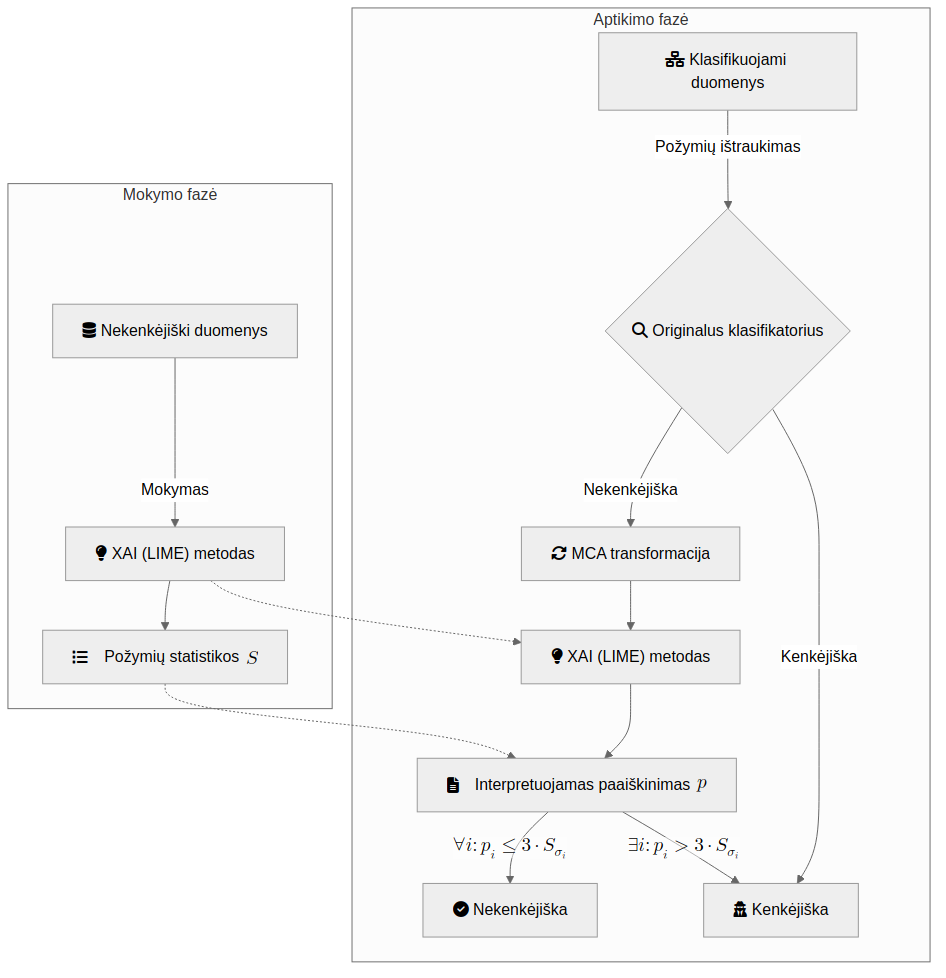
\includegraphics[width=0.95\textwidth]{images/original.png}
        \caption{\LIME ir \gls{mca} sintezės \gls{ae} aptikimo metodo iliustracija}
        \label{fig:original}
    \end{minipage}
    \begin{minipage}{0.48\textwidth}
        \centering
        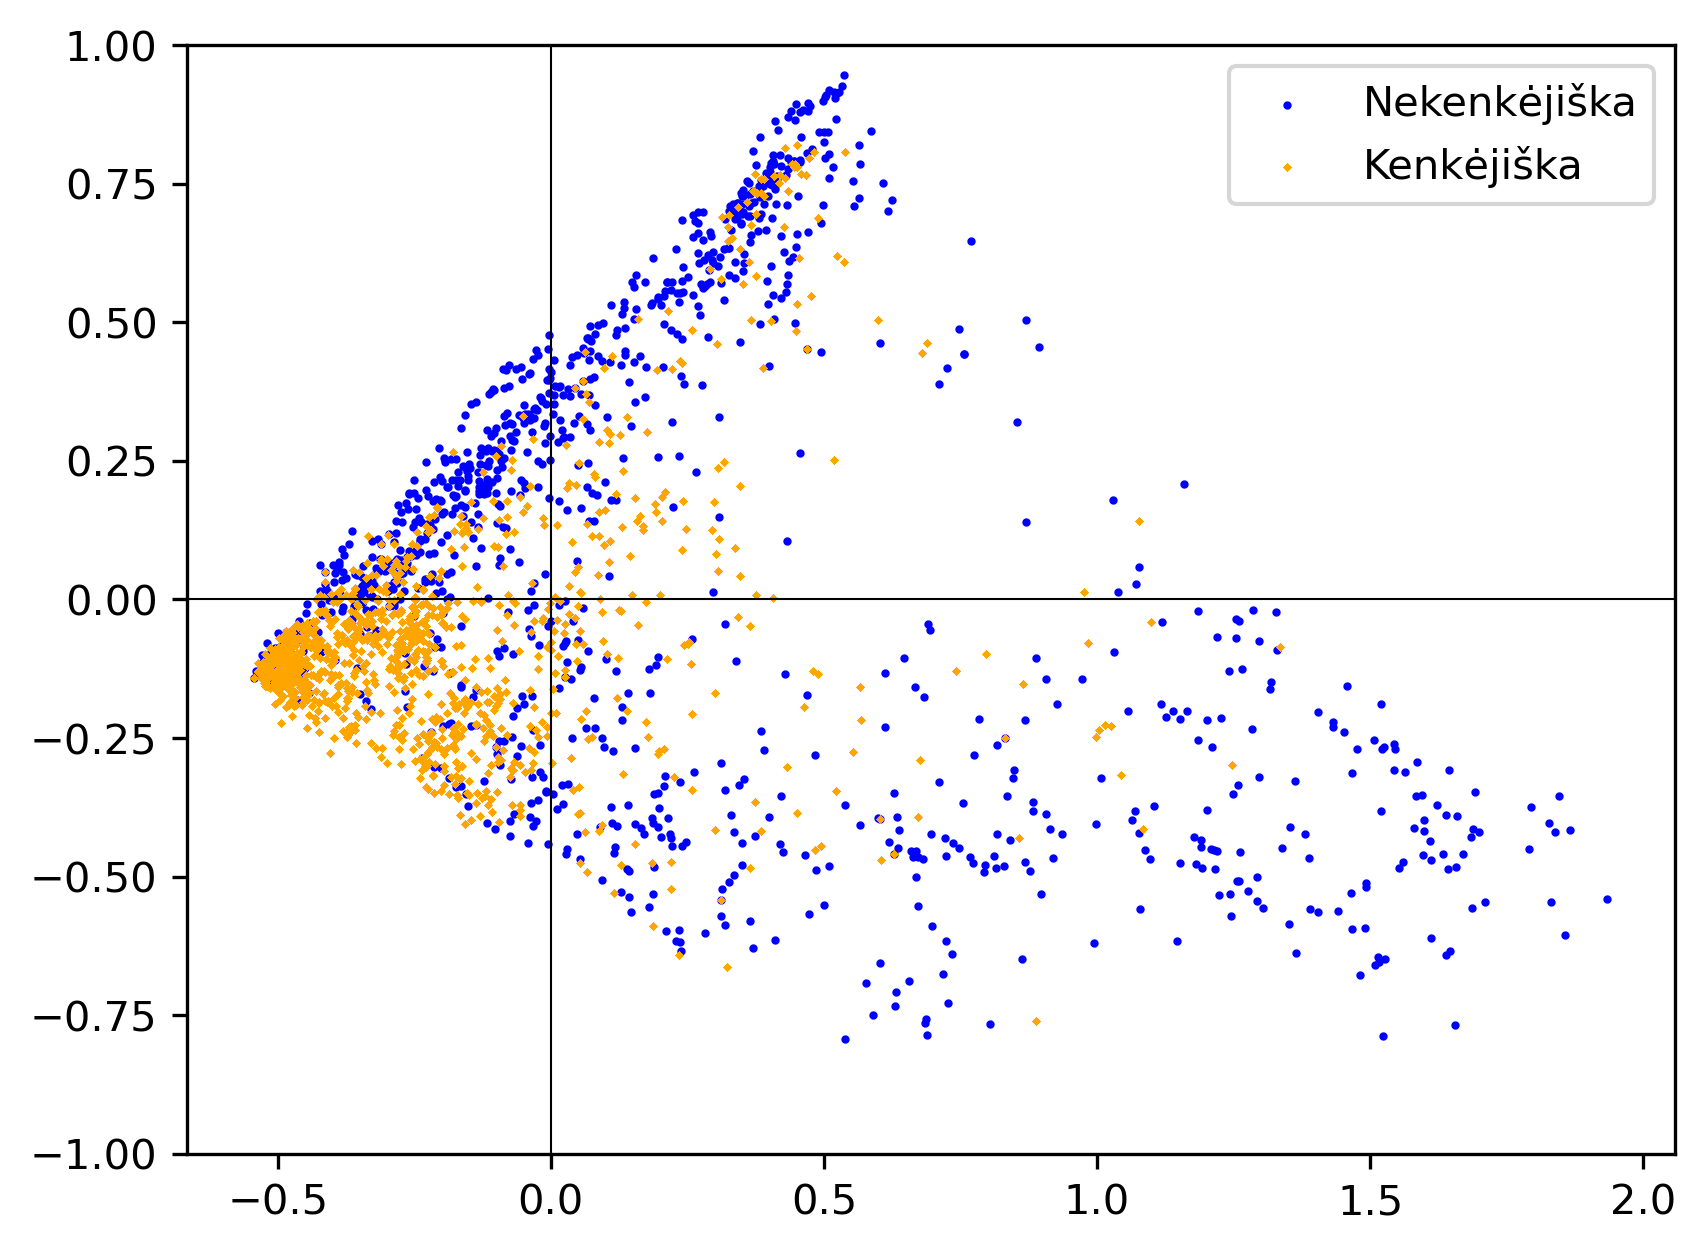
\includegraphics[width=\textwidth]{images/mca_scatter.png}
        \caption{Pirmųjų dviejų \gls{mca} transformacijos komponenčių pavyzdys}
        \label{fig:scree}
    \end{minipage}
\end{figure}


% Problem with selecting N components to explain
% Problem with binary feature vectors
% Synthesis of MCA and LIME (original)
% Method flow diagram (adaptation)
% Importance of keeping obfuscation detection hidden (original)